\documentclass[twoside]{book}

% Packages required by doxygen
\usepackage{fixltx2e}
\usepackage{calc}
\usepackage{doxygen}
\usepackage[export]{adjustbox} % also loads graphicx
\usepackage{graphicx}
\usepackage[utf8]{inputenc}
\usepackage{makeidx}
\usepackage{multicol}
\usepackage{multirow}
\PassOptionsToPackage{warn}{textcomp}
\usepackage{textcomp}
\usepackage[nointegrals]{wasysym}
\usepackage[table]{xcolor}

% Font selection
\usepackage[T1]{fontenc}
\usepackage[scaled=.90]{helvet}
\usepackage{courier}
\usepackage{amssymb}
\usepackage{sectsty}
\renewcommand{\familydefault}{\sfdefault}
\allsectionsfont{%
  \fontseries{bc}\selectfont%
  \color{darkgray}%
}
\renewcommand{\DoxyLabelFont}{%
  \fontseries{bc}\selectfont%
  \color{darkgray}%
}
\newcommand{\+}{\discretionary{\mbox{\scriptsize$\hookleftarrow$}}{}{}}

% Page & text layout
\usepackage{geometry}
\geometry{%
  a4paper,%
  top=2.5cm,%
  bottom=2.5cm,%
  left=2.5cm,%
  right=2.5cm%
}
\tolerance=750
\hfuzz=15pt
\hbadness=750
\setlength{\emergencystretch}{15pt}
\setlength{\parindent}{0cm}
\setlength{\parskip}{3ex plus 2ex minus 2ex}
\makeatletter
\renewcommand{\paragraph}{%
  \@startsection{paragraph}{4}{0ex}{-1.0ex}{1.0ex}{%
    \normalfont\normalsize\bfseries\SS@parafont%
  }%
}
\renewcommand{\subparagraph}{%
  \@startsection{subparagraph}{5}{0ex}{-1.0ex}{1.0ex}{%
    \normalfont\normalsize\bfseries\SS@subparafont%
  }%
}
\makeatother

% Headers & footers
\usepackage{fancyhdr}
\pagestyle{fancyplain}
\fancyhead[LE]{\fancyplain{}{\bfseries\thepage}}
\fancyhead[CE]{\fancyplain{}{}}
\fancyhead[RE]{\fancyplain{}{\bfseries\leftmark}}
\fancyhead[LO]{\fancyplain{}{\bfseries\rightmark}}
\fancyhead[CO]{\fancyplain{}{}}
\fancyhead[RO]{\fancyplain{}{\bfseries\thepage}}
\fancyfoot[LE]{\fancyplain{}{}}
\fancyfoot[CE]{\fancyplain{}{}}
\fancyfoot[RE]{\fancyplain{}{\bfseries\scriptsize Generated by Doxygen }}
\fancyfoot[LO]{\fancyplain{}{\bfseries\scriptsize Generated by Doxygen }}
\fancyfoot[CO]{\fancyplain{}{}}
\fancyfoot[RO]{\fancyplain{}{}}
\renewcommand{\footrulewidth}{0.4pt}
\renewcommand{\chaptermark}[1]{%
  \markboth{#1}{}%
}
\renewcommand{\sectionmark}[1]{%
  \markright{\thesection\ #1}%
}

% Indices & bibliography
\usepackage{natbib}
\usepackage[titles]{tocloft}
\setcounter{tocdepth}{3}
\setcounter{secnumdepth}{5}
\makeindex

% Hyperlinks (required, but should be loaded last)
\usepackage{ifpdf}
\ifpdf
  \usepackage[pdftex,pagebackref=true]{hyperref}
\else
  \usepackage[ps2pdf,pagebackref=true]{hyperref}
\fi
\hypersetup{%
  colorlinks=true,%
  linkcolor=blue,%
  citecolor=blue,%
  unicode%
}

% Custom commands
\newcommand{\clearemptydoublepage}{%
  \newpage{\pagestyle{empty}\cleardoublepage}%
}

\usepackage{caption}
\captionsetup{labelsep=space,justification=centering,font={bf},singlelinecheck=off,skip=4pt,position=top}

%===== C O N T E N T S =====

\begin{document}

% Titlepage & ToC
\hypersetup{pageanchor=false,
             bookmarksnumbered=true,
             pdfencoding=unicode
            }
\pagenumbering{alph}
\begin{titlepage}
\vspace*{7cm}
\begin{center}%
{\Large I\+G2-\/\+Battle\+Cruiser-\/\+Client \\[1ex]\large 1.\+0 }\\
\vspace*{1cm}
{\large Generated by Doxygen 1.8.13}\\
\end{center}
\end{titlepage}
\clearemptydoublepage
\pagenumbering{roman}
\tableofcontents
\clearemptydoublepage
\pagenumbering{arabic}
\hypersetup{pageanchor=true}

%--- Begin generated contents ---
\chapter{Data Structure Index}
\section{Data Structures}
Here are the data structures with brief descriptions\+:\begin{DoxyCompactList}
\item\contentsline{section}{\hyperlink{structgame_cell}{game\+Cell} }{\pageref{structgame_cell}}{}
\item\contentsline{section}{\hyperlink{structmouse_pos}{mouse\+Pos} }{\pageref{structmouse_pos}}{}
\item\contentsline{section}{\hyperlink{structnet_connection_info}{net\+Connection\+Info} }{\pageref{structnet_connection_info}}{}
\item\contentsline{section}{\hyperlink{structnet_packet}{net\+Packet} }{\pageref{structnet_packet}}{}
\end{DoxyCompactList}

\chapter{File Index}
\section{File List}
Here is a list of all documented files with brief descriptions\+:\begin{DoxyCompactList}
\item\contentsline{section}{includes/\hyperlink{clt_net_8h}{clt\+Net.\+h} \\*Déclaration pour la lib networking }{\pageref{clt_net_8h}}{}
\item\contentsline{section}{includes/\hyperlink{game_8h}{game.\+h} \\*Déclaration pour le jeu }{\pageref{game_8h}}{}
\item\contentsline{section}{includes/\hyperlink{game_cell_8h}{game\+Cell.\+h} \\*Déclaration pour les cases de jeu }{\pageref{game_cell_8h}}{}
\item\contentsline{section}{src/{\bfseries app.\+c} }{\pageref{app_8c}}{}
\item\contentsline{section}{src/{\bfseries game.\+c} }{\pageref{game_8c}}{}
\item\contentsline{section}{src/{\bfseries game\+Cell.\+c} }{\pageref{game_cell_8c}}{}
\item\contentsline{section}{src/{\bfseries net.\+c} }{\pageref{net_8c}}{}
\end{DoxyCompactList}

\chapter{Data Structure Documentation}
\hypertarget{structgame_cell}{}\section{game\+Cell Struct Reference}
\label{structgame_cell}\index{game\+Cell@{game\+Cell}}
\subsection*{Data Fields}
\begin{DoxyCompactItemize}
\item 
\mbox{\Hypertarget{structgame_cell_a55aefd071649ac9dd8133e2d8a52d11f}\label{structgame_cell_a55aefd071649ac9dd8133e2d8a52d11f}} 
S\+D\+L\+\_\+\+Rect {\bfseries rect}
\item 
\mbox{\Hypertarget{structgame_cell_a058f4c912c8378ad76523861b1e0ad4b}\label{structgame_cell_a058f4c912c8378ad76523861b1e0ad4b}} 
enum \hyperlink{game_cell_8h_a38e97bf4503f8099c49fac77b951ae63}{cell\+State} {\bfseries state}
\item 
\mbox{\Hypertarget{structgame_cell_a9dda3ce5e0a6197a2a5a675340b1e1cb}\label{structgame_cell_a9dda3ce5e0a6197a2a5a675340b1e1cb}} 
u\+\_\+int8\+\_\+t {\bfseries has\+Ship}
\end{DoxyCompactItemize}


\subsection{Detailed Description}


Definition at line 36 of file game\+Cell.\+h.



The documentation for this struct was generated from the following file\+:\begin{DoxyCompactItemize}
\item 
includes/\hyperlink{game_cell_8h}{game\+Cell.\+h}\end{DoxyCompactItemize}

\hypertarget{structmouse_pos}{}\section{mouse\+Pos Struct Reference}
\label{structmouse_pos}\index{mouse\+Pos@{mouse\+Pos}}


{\ttfamily \#include $<$game.\+h$>$}

\subsection*{Data Fields}
\begin{DoxyCompactItemize}
\item 
\mbox{\Hypertarget{structmouse_pos_a121a1c4a169f06c39e7d987484676ca1}\label{structmouse_pos_a121a1c4a169f06c39e7d987484676ca1}} 
u\+\_\+int8\+\_\+t {\bfseries x}
\item 
\mbox{\Hypertarget{structmouse_pos_ab1f68b8e03b9be58dc27625ca64d3687}\label{structmouse_pos_ab1f68b8e03b9be58dc27625ca64d3687}} 
u\+\_\+int8\+\_\+t {\bfseries y}
\end{DoxyCompactItemize}


\subsection{Detailed Description}
Structure représentant la position de la souris à l\textquotesingle{}intérieur de la grille de jeu 

Definition at line 31 of file game.\+h.



The documentation for this struct was generated from the following file\+:\begin{DoxyCompactItemize}
\item 
includes/\hyperlink{game_8h}{game.\+h}\end{DoxyCompactItemize}

\hypertarget{structnet_connection_info}{}\section{net\+Connection\+Info Struct Reference}
\label{structnet_connection_info}\index{net\+Connection\+Info@{net\+Connection\+Info}}
\subsection*{Data Fields}
\begin{DoxyCompactItemize}
\item 
\mbox{\Hypertarget{structnet_connection_info_a9e26a4afe91a21810290057677a17a11}\label{structnet_connection_info_a9e26a4afe91a21810290057677a17a11}} 
u\+\_\+int16\+\_\+t {\bfseries port}
\item 
\mbox{\Hypertarget{structnet_connection_info_ad540706412769097e113feb208f0b6bf}\label{structnet_connection_info_ad540706412769097e113feb208f0b6bf}} 
char $\ast$ {\bfseries ipaddr}
\end{DoxyCompactItemize}


\subsection{Detailed Description}


Definition at line 45 of file clt\+Net.\+h.



The documentation for this struct was generated from the following file\+:\begin{DoxyCompactItemize}
\item 
includes/\hyperlink{clt_net_8h}{clt\+Net.\+h}\end{DoxyCompactItemize}

\hypertarget{structnet_packet}{}\section{net\+Packet Struct Reference}
\label{structnet_packet}\index{net\+Packet@{net\+Packet}}
\subsection*{Data Fields}
\begin{DoxyCompactItemize}
\item 
\mbox{\Hypertarget{structnet_packet_a175de41b73096984ed32e887e5df63e7}\label{structnet_packet_a175de41b73096984ed32e887e5df63e7}} 
int8\+\_\+t {\bfseries size}
\item 
\mbox{\Hypertarget{structnet_packet_acfe36f8cabae4902ccb7605df9ad0f8d}\label{structnet_packet_acfe36f8cabae4902ccb7605df9ad0f8d}} 
u\+\_\+int8\+\_\+t {\bfseries flag}
\item 
\mbox{\Hypertarget{structnet_packet_a7127c16b9b3b7f75d2dda2420d88c48f}\label{structnet_packet_a7127c16b9b3b7f75d2dda2420d88c48f}} 
u\+\_\+int8\+\_\+t {\bfseries data} \mbox{[}20\mbox{]}
\end{DoxyCompactItemize}


\subsection{Detailed Description}


Definition at line 34 of file clt\+Net.\+h.



The documentation for this struct was generated from the following file\+:\begin{DoxyCompactItemize}
\item 
includes/\hyperlink{clt_net_8h}{clt\+Net.\+h}\end{DoxyCompactItemize}

\chapter{File Documentation}
\hypertarget{clt_net_8h}{}\section{includes/clt\+Net.h File Reference}
\label{clt_net_8h}\index{includes/clt\+Net.\+h@{includes/clt\+Net.\+h}}


Déclaration pour la lib networking.  


{\ttfamily \#include \char`\"{}../../shared/includes.\+h\char`\"{}}\newline
{\ttfamily \#include $<$poll.\+h$>$}\newline
Include dependency graph for clt\+Net.\+h\+:
\nopagebreak
\begin{figure}[H]
\begin{center}
\leavevmode
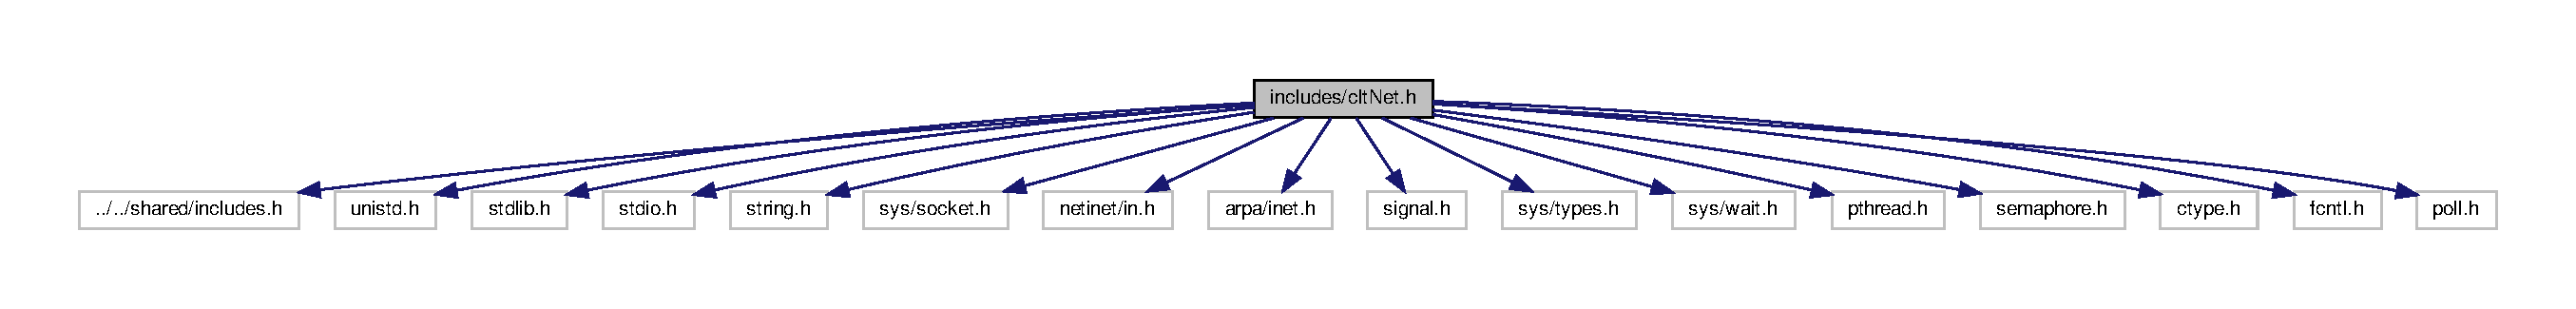
\includegraphics[width=350pt]{clt_net_8h__incl}
\end{center}
\end{figure}
This graph shows which files directly or indirectly include this file\+:
\nopagebreak
\begin{figure}[H]
\begin{center}
\leavevmode
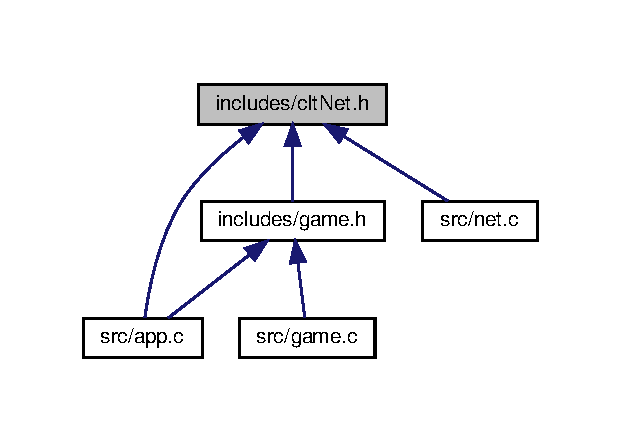
\includegraphics[width=298pt]{clt_net_8h__dep__incl}
\end{center}
\end{figure}
\subsection*{Data Structures}
\begin{DoxyCompactItemize}
\item 
struct \hyperlink{structnet_packet}{net\+Packet}
\item 
struct \hyperlink{structnet_connection_info}{net\+Connection\+Info}
\end{DoxyCompactItemize}
\subsection*{Macros}
\begin{DoxyCompactItemize}
\item 
\#define \hyperlink{clt_net_8h_ac42367fe5c999ec6650de83e9d72fe8c}{S\+E\+R\+V\+E\+R\+\_\+\+P\+O\+RT}~6666
\item 
\#define \hyperlink{clt_net_8h_adfe214cdf99ea5f07a40e6e322939dd9}{R\+E\+A\+D\+\_\+\+TO}~500
\end{DoxyCompactItemize}
\subsection*{Typedefs}
\begin{DoxyCompactItemize}
\item 
\mbox{\Hypertarget{clt_net_8h_ab6549bcbc223bcbd6c7e4b513f1f236a}\label{clt_net_8h_ab6549bcbc223bcbd6c7e4b513f1f236a}} 
typedef struct \hyperlink{structnet_packet}{net\+Packet} {\bfseries packet\+\_\+t}
\item 
\mbox{\Hypertarget{clt_net_8h_ada51de97305197df8958c1591e64b068}\label{clt_net_8h_ada51de97305197df8958c1591e64b068}} 
typedef struct \hyperlink{structnet_connection_info}{net\+Connection\+Info} {\bfseries connection\+Info\+\_\+t}
\end{DoxyCompactItemize}
\subsection*{Functions}
\begin{DoxyCompactItemize}
\item 
void \hyperlink{clt_net_8h_a4d9220d85eee06ac4b2205196126953f}{create\+Server} ()
\item 
void \hyperlink{clt_net_8h_a0dcd7a35d526d4014f56a18dc4a0494a}{join\+Server} (\hyperlink{structnet_connection_info}{connection\+Info\+\_\+t} $\ast$)
\item 
void \hyperlink{clt_net_8h_ad99a2f323b9c39be8a81a6057ff3d717}{close\+Server} ()
\item 
void \hyperlink{clt_net_8h_abe175fcf658475bc56e9d6fa02bc88ec}{disconnect} ()
\item 
void \hyperlink{clt_net_8h_a068e6bafd1f6441a0f8b6aea130fdcc8}{net\+Send} (\hyperlink{structnet_packet}{packet\+\_\+t})
\item 
\hyperlink{structnet_packet}{packet\+\_\+t} \hyperlink{clt_net_8h_af91a05c6e75309e686e6a24fc9e11637}{net\+Read} ()
\item 
u\+\_\+int8\+\_\+t \hyperlink{clt_net_8h_a4770fcff580d18f4f92ac1d9fbc93097}{is\+Host} ()
\item 
u\+\_\+int8\+\_\+t \hyperlink{clt_net_8h_af160f7fbbf281d018ae3162521b8267d}{is\+Connected} ()
\item 
u\+\_\+int8\+\_\+t \hyperlink{clt_net_8h_a3482ef4e4b21925e27b60f77d60b6cd1}{has\+Client} ()
\end{DoxyCompactItemize}


\subsection{Detailed Description}
Déclaration pour la lib networking. 

\begin{DoxyAuthor}{Author}
Thomas De Maen 
\end{DoxyAuthor}
\begin{DoxyVersion}{Version}
1.\+0 
\end{DoxyVersion}
\begin{DoxyDate}{Date}
14 Janvier 2020
\end{DoxyDate}
Il s\textquotesingle{}agit du fichier de délaration des différentes structures de données et fonctions utilisées pour le bon fonctionnement de la librairie Networking. 

\subsection{Macro Definition Documentation}
\mbox{\Hypertarget{clt_net_8h_adfe214cdf99ea5f07a40e6e322939dd9}\label{clt_net_8h_adfe214cdf99ea5f07a40e6e322939dd9}} 
\index{clt\+Net.\+h@{clt\+Net.\+h}!R\+E\+A\+D\+\_\+\+TO@{R\+E\+A\+D\+\_\+\+TO}}
\index{R\+E\+A\+D\+\_\+\+TO@{R\+E\+A\+D\+\_\+\+TO}!clt\+Net.\+h@{clt\+Net.\+h}}
\subsubsection{\texorpdfstring{R\+E\+A\+D\+\_\+\+TO}{READ\_TO}}
{\footnotesize\ttfamily \#define R\+E\+A\+D\+\_\+\+TO~500}

Nombre de milisecondes avant qu\textquotesingle{}une opération de lecture time out 

Definition at line 27 of file clt\+Net.\+h.

\mbox{\Hypertarget{clt_net_8h_ac42367fe5c999ec6650de83e9d72fe8c}\label{clt_net_8h_ac42367fe5c999ec6650de83e9d72fe8c}} 
\index{clt\+Net.\+h@{clt\+Net.\+h}!S\+E\+R\+V\+E\+R\+\_\+\+P\+O\+RT@{S\+E\+R\+V\+E\+R\+\_\+\+P\+O\+RT}}
\index{S\+E\+R\+V\+E\+R\+\_\+\+P\+O\+RT@{S\+E\+R\+V\+E\+R\+\_\+\+P\+O\+RT}!clt\+Net.\+h@{clt\+Net.\+h}}
\subsubsection{\texorpdfstring{S\+E\+R\+V\+E\+R\+\_\+\+P\+O\+RT}{SERVER\_PORT}}
{\footnotesize\ttfamily \#define S\+E\+R\+V\+E\+R\+\_\+\+P\+O\+RT~6666}

Numéro de port de l\textquotesingle{}hôte d\textquotesingle{}une partie 

Definition at line 21 of file clt\+Net.\+h.



\subsection{Function Documentation}
\mbox{\Hypertarget{clt_net_8h_ad99a2f323b9c39be8a81a6057ff3d717}\label{clt_net_8h_ad99a2f323b9c39be8a81a6057ff3d717}} 
\index{clt\+Net.\+h@{clt\+Net.\+h}!close\+Server@{close\+Server}}
\index{close\+Server@{close\+Server}!clt\+Net.\+h@{clt\+Net.\+h}}
\subsubsection{\texorpdfstring{close\+Server()}{closeServer()}}
{\footnotesize\ttfamily close\+Server (\begin{DoxyParamCaption}\item[{void}]{ }\end{DoxyParamCaption})}

Fonction permettant à l\textquotesingle{}hôte de fermer son serveur 

Definition at line 149 of file net.\+c.

\mbox{\Hypertarget{clt_net_8h_a4d9220d85eee06ac4b2205196126953f}\label{clt_net_8h_a4d9220d85eee06ac4b2205196126953f}} 
\index{clt\+Net.\+h@{clt\+Net.\+h}!create\+Server@{create\+Server}}
\index{create\+Server@{create\+Server}!clt\+Net.\+h@{clt\+Net.\+h}}
\subsubsection{\texorpdfstring{create\+Server()}{createServer()}}
{\footnotesize\ttfamily create\+Server (\begin{DoxyParamCaption}\item[{void}]{ }\end{DoxyParamCaption})}

Fonction permettant à une application cliente d\textquotesingle{}héberger une partie en P2P 

Definition at line 127 of file net.\+c.

\mbox{\Hypertarget{clt_net_8h_abe175fcf658475bc56e9d6fa02bc88ec}\label{clt_net_8h_abe175fcf658475bc56e9d6fa02bc88ec}} 
\index{clt\+Net.\+h@{clt\+Net.\+h}!disconnect@{disconnect}}
\index{disconnect@{disconnect}!clt\+Net.\+h@{clt\+Net.\+h}}
\subsubsection{\texorpdfstring{disconnect()}{disconnect()}}
{\footnotesize\ttfamily disconnect (\begin{DoxyParamCaption}\item[{void}]{ }\end{DoxyParamCaption})}

Fonction permettant à un client de se déconnecter d\textquotesingle{}un hôte 

Definition at line 159 of file net.\+c.

\mbox{\Hypertarget{clt_net_8h_a3482ef4e4b21925e27b60f77d60b6cd1}\label{clt_net_8h_a3482ef4e4b21925e27b60f77d60b6cd1}} 
\index{clt\+Net.\+h@{clt\+Net.\+h}!has\+Client@{has\+Client}}
\index{has\+Client@{has\+Client}!clt\+Net.\+h@{clt\+Net.\+h}}
\subsubsection{\texorpdfstring{has\+Client()}{hasClient()}}
{\footnotesize\ttfamily has\+Client (\begin{DoxyParamCaption}\item[{void}]{ }\end{DoxyParamCaption})}

Fonction permettant à une application cliente de savoir si elle a des clients connectés \begin{DoxyReturn}{Returns}
1 si l\textquotesingle{}appellant est un hôte avec au moins un client connecté et 0 sinon 
\end{DoxyReturn}


Definition at line 212 of file net.\+c.

\mbox{\Hypertarget{clt_net_8h_af160f7fbbf281d018ae3162521b8267d}\label{clt_net_8h_af160f7fbbf281d018ae3162521b8267d}} 
\index{clt\+Net.\+h@{clt\+Net.\+h}!is\+Connected@{is\+Connected}}
\index{is\+Connected@{is\+Connected}!clt\+Net.\+h@{clt\+Net.\+h}}
\subsubsection{\texorpdfstring{is\+Connected()}{isConnected()}}
{\footnotesize\ttfamily is\+Connected (\begin{DoxyParamCaption}\item[{void}]{ }\end{DoxyParamCaption})}

Fonction permettant à une application de savoir si elle est connectée \begin{DoxyReturn}{Returns}
1 si l\textquotesingle{}appellant est connecté (ou est l\textquotesingle{}hôte) à un serveur et 0 sinon 
\end{DoxyReturn}


Definition at line 208 of file net.\+c.

\mbox{\Hypertarget{clt_net_8h_a4770fcff580d18f4f92ac1d9fbc93097}\label{clt_net_8h_a4770fcff580d18f4f92ac1d9fbc93097}} 
\index{clt\+Net.\+h@{clt\+Net.\+h}!is\+Host@{is\+Host}}
\index{is\+Host@{is\+Host}!clt\+Net.\+h@{clt\+Net.\+h}}
\subsubsection{\texorpdfstring{is\+Host()}{isHost()}}
{\footnotesize\ttfamily is\+Host (\begin{DoxyParamCaption}\item[{void}]{ }\end{DoxyParamCaption})}

Fonction permettant à une application cliente de savoir si elle est hôte \begin{DoxyReturn}{Returns}
1 si l\textquotesingle{}appellant est l\textquotesingle{}hôte d\textquotesingle{}un serveur et 0 sinon 
\end{DoxyReturn}


Definition at line 204 of file net.\+c.

\mbox{\Hypertarget{clt_net_8h_a0dcd7a35d526d4014f56a18dc4a0494a}\label{clt_net_8h_a0dcd7a35d526d4014f56a18dc4a0494a}} 
\index{clt\+Net.\+h@{clt\+Net.\+h}!join\+Server@{join\+Server}}
\index{join\+Server@{join\+Server}!clt\+Net.\+h@{clt\+Net.\+h}}
\subsubsection{\texorpdfstring{join\+Server()}{joinServer()}}
{\footnotesize\ttfamily join\+Server (\begin{DoxyParamCaption}\item[{\hyperlink{structnet_connection_info}{connection\+Info\+\_\+t} $\ast$}]{p\+Infos }\end{DoxyParamCaption})}

Fonction permettant à une application cliente de rejoindre une partie hébergée 
\begin{DoxyParams}{Parameters}
{\em p\+Infos} & Pointeur sur les informations de connexion au serveur \\
\hline
\end{DoxyParams}


Definition at line 138 of file net.\+c.

\mbox{\Hypertarget{clt_net_8h_af91a05c6e75309e686e6a24fc9e11637}\label{clt_net_8h_af91a05c6e75309e686e6a24fc9e11637}} 
\index{clt\+Net.\+h@{clt\+Net.\+h}!net\+Read@{net\+Read}}
\index{net\+Read@{net\+Read}!clt\+Net.\+h@{clt\+Net.\+h}}
\subsubsection{\texorpdfstring{net\+Read()}{netRead()}}
{\footnotesize\ttfamily net\+Read (\begin{DoxyParamCaption}\item[{void}]{ }\end{DoxyParamCaption})}

Fonction permettant de lire des données depuis le réseau, il est nécessaire qu\textquotesingle{}une connexion soit active afin d\textquotesingle{}être utilisée \begin{DoxyReturn}{Returns}
Le paquet qui a été lu depuis une connexion T\+CP 
\end{DoxyReturn}


Definition at line 182 of file net.\+c.

\mbox{\Hypertarget{clt_net_8h_a068e6bafd1f6441a0f8b6aea130fdcc8}\label{clt_net_8h_a068e6bafd1f6441a0f8b6aea130fdcc8}} 
\index{clt\+Net.\+h@{clt\+Net.\+h}!net\+Send@{net\+Send}}
\index{net\+Send@{net\+Send}!clt\+Net.\+h@{clt\+Net.\+h}}
\subsubsection{\texorpdfstring{net\+Send()}{netSend()}}
{\footnotesize\ttfamily net\+Send (\begin{DoxyParamCaption}\item[{\hyperlink{structnet_packet}{packet\+\_\+t}}]{p }\end{DoxyParamCaption})}

Fonction permettant d\textquotesingle{}envoyer des données sur le réseau, il est nécessaire qu\textquotesingle{}une connexion soit active afin d\textquotesingle{}être utilisée 
\begin{DoxyParams}{Parameters}
{\em p} & Paquet à envoyer au travers d\textquotesingle{}une connexion T\+CP \\
\hline
\end{DoxyParams}


Definition at line 168 of file net.\+c.


\hypertarget{game_8h}{}\section{includes/game.h File Reference}
\label{game_8h}\index{includes/game.\+h@{includes/game.\+h}}


Déclaration pour le jeu.  


{\ttfamily \#include $<$S\+D\+L2/\+S\+D\+L.\+h$>$}\newline
{\ttfamily \#include \char`\"{}../includes/clt\+Net.\+h\char`\"{}}\newline
Include dependency graph for game.\+h\+:
\nopagebreak
\begin{figure}[H]
\begin{center}
\leavevmode
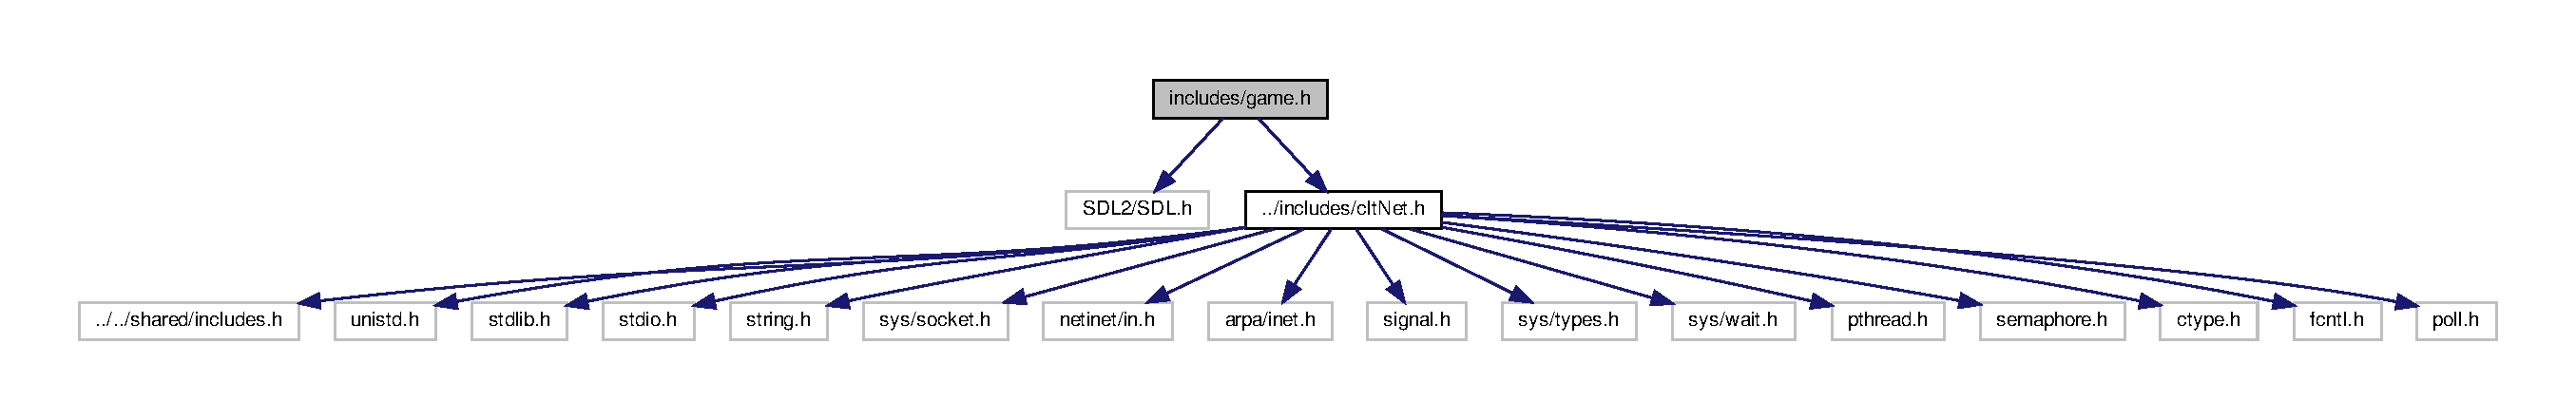
\includegraphics[width=350pt]{game_8h__incl}
\end{center}
\end{figure}
This graph shows which files directly or indirectly include this file\+:
\nopagebreak
\begin{figure}[H]
\begin{center}
\leavevmode
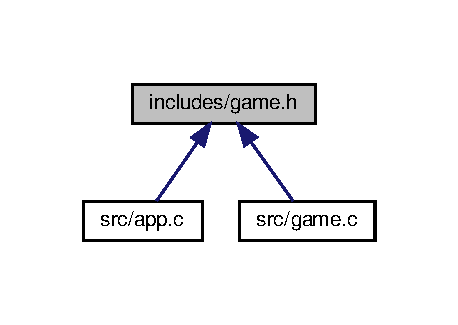
\includegraphics[width=220pt]{game_8h__dep__incl}
\end{center}
\end{figure}
\subsection*{Data Structures}
\begin{DoxyCompactItemize}
\item 
struct \hyperlink{structmouse_pos}{mouse\+Pos}
\end{DoxyCompactItemize}
\subsection*{Typedefs}
\begin{DoxyCompactItemize}
\item 
\mbox{\Hypertarget{game_8h_ac601b8bdcae724f2d2745e0dc8656d47}\label{game_8h_ac601b8bdcae724f2d2745e0dc8656d47}} 
typedef struct \hyperlink{structmouse_pos}{mouse\+Pos} {\bfseries t\+\_\+mouse\+Pos}
\end{DoxyCompactItemize}
\subsection*{Enumerations}
\begin{DoxyCompactItemize}
\item 
enum \hyperlink{game_8h_aaf29bbe309504beb4cfec2481eacee62}{game\+State} \{ {\bfseries M\+A\+I\+N\+\_\+\+M\+E\+NU}, 
{\bfseries P\+L\+A\+C\+I\+NG}, 
{\bfseries P\+L\+A\+Y\+I\+NG}
 \}
\end{DoxyCompactItemize}
\subsection*{Functions}
\begin{DoxyCompactItemize}
\item 
void \hyperlink{game_8h_a41ac2567d4645c7f92a1ad44194a02e0}{game\+Init} ()
\item 
void \hyperlink{game_8h_a46b6e5d99fee9b3daccde93b291baede}{game\+Update} ()
\item 
void \hyperlink{game_8h_a18498e6ffe8b6ccd129f2c416a9a2c97}{game\+Draw} (S\+D\+L\+\_\+\+Renderer $\ast$)
\item 
void \hyperlink{game_8h_acb3f0314332e44f50b8a08d97ae74509}{game\+Mouse\+Event} (S\+D\+L\+\_\+\+Mouse\+Button\+Event)
\item 
void \hyperlink{game_8h_aee864b1d56e4d7217c14e8ab69a783bc}{game\+Mouse\+Motion} (S\+D\+L\+\_\+\+Mouse\+Motion\+Event)
\item 
void \hyperlink{game_8h_aa53e39913b7b9af45ad49c3bf1b75ac5}{game\+Key\+Pressed} (S\+D\+L\+\_\+\+Keyboard\+Event)
\item 
int \hyperlink{game_8h_af15d7f4d0494afa16263d231aba7e094}{min} (int, int)
\end{DoxyCompactItemize}


\subsection{Detailed Description}
Déclaration pour le jeu. 

\begin{DoxyAuthor}{Author}
Thomas De Maen 
\end{DoxyAuthor}
\begin{DoxyVersion}{Version}
1.\+0 
\end{DoxyVersion}
\begin{DoxyDate}{Date}
14 Janvier 2020
\end{DoxyDate}
Il s\textquotesingle{}agit du fichier de délaration des différentes structures de données et fonctions utilisées pour le bon fonctionnement du jeu. 

\subsection{Enumeration Type Documentation}
\mbox{\Hypertarget{game_8h_aaf29bbe309504beb4cfec2481eacee62}\label{game_8h_aaf29bbe309504beb4cfec2481eacee62}} 
\index{game.\+h@{game.\+h}!game\+State@{game\+State}}
\index{game\+State@{game\+State}!game.\+h@{game.\+h}}
\subsubsection{\texorpdfstring{game\+State}{gameState}}
{\footnotesize\ttfamily enum \hyperlink{game_8h_aaf29bbe309504beb4cfec2481eacee62}{game\+State}}

Enum représentant les différents états possibles du jeu 

Definition at line 21 of file game.\+h.



\subsection{Function Documentation}
\mbox{\Hypertarget{game_8h_a18498e6ffe8b6ccd129f2c416a9a2c97}\label{game_8h_a18498e6ffe8b6ccd129f2c416a9a2c97}} 
\index{game.\+h@{game.\+h}!game\+Draw@{game\+Draw}}
\index{game\+Draw@{game\+Draw}!game.\+h@{game.\+h}}
\subsubsection{\texorpdfstring{game\+Draw()}{gameDraw()}}
{\footnotesize\ttfamily game\+Draw (\begin{DoxyParamCaption}\item[{S\+D\+L\+\_\+\+Renderer $\ast$}]{p\+Rend }\end{DoxyParamCaption})}

Fonction appellée en continue afin de dessiner le jeu, elle est appellée après chaque update T\+O\+DO\+: Réguler la fréquence de rafraichissement (F\+PS cap) 
\begin{DoxyParams}{Parameters}
{\em p\+Rend} & Pointeur sur le renderer utilisé par S\+DL pour dessiner sur la fenêtre de jeu \\
\hline
\end{DoxyParams}


Definition at line 160 of file game.\+c.

\mbox{\Hypertarget{game_8h_a41ac2567d4645c7f92a1ad44194a02e0}\label{game_8h_a41ac2567d4645c7f92a1ad44194a02e0}} 
\index{game.\+h@{game.\+h}!game\+Init@{game\+Init}}
\index{game\+Init@{game\+Init}!game.\+h@{game.\+h}}
\subsubsection{\texorpdfstring{game\+Init()}{gameInit()}}
{\footnotesize\ttfamily game\+Init (\begin{DoxyParamCaption}\item[{void}]{ }\end{DoxyParamCaption})}

Fonction appellée après l\textquotesingle{}initialisation de la S\+DL et la création de la fenêtre Le premier entier permet de savoir si le client est un hôte ou non, dans le cas où ce n\textquotesingle{}est pas l\textquotesingle{}hôte, les infos de connexion sont passés en deuxième argument 

Definition at line 22 of file game.\+c.

\mbox{\Hypertarget{game_8h_aa53e39913b7b9af45ad49c3bf1b75ac5}\label{game_8h_aa53e39913b7b9af45ad49c3bf1b75ac5}} 
\index{game.\+h@{game.\+h}!game\+Key\+Pressed@{game\+Key\+Pressed}}
\index{game\+Key\+Pressed@{game\+Key\+Pressed}!game.\+h@{game.\+h}}
\subsubsection{\texorpdfstring{game\+Key\+Pressed()}{gameKeyPressed()}}
{\footnotesize\ttfamily game\+Key\+Pressed (\begin{DoxyParamCaption}\item[{S\+D\+L\+\_\+\+Keyboard\+Event}]{e }\end{DoxyParamCaption})}

Fonction appellée à chaque fois qu\textquotesingle{}un événement du type S\+D\+L\+\_\+\+K\+E\+Y\+D\+O\+WN est récupéré par S\+DL 
\begin{DoxyParams}{Parameters}
{\em e} & Evénement capturé par S\+DL \\
\hline
\end{DoxyParams}


Definition at line 248 of file game.\+c.

\mbox{\Hypertarget{game_8h_acb3f0314332e44f50b8a08d97ae74509}\label{game_8h_acb3f0314332e44f50b8a08d97ae74509}} 
\index{game.\+h@{game.\+h}!game\+Mouse\+Event@{game\+Mouse\+Event}}
\index{game\+Mouse\+Event@{game\+Mouse\+Event}!game.\+h@{game.\+h}}
\subsubsection{\texorpdfstring{game\+Mouse\+Event()}{gameMouseEvent()}}
{\footnotesize\ttfamily game\+Mouse\+Event (\begin{DoxyParamCaption}\item[{S\+D\+L\+\_\+\+Mouse\+Button\+Event}]{e }\end{DoxyParamCaption})}

Fonction appellée à chaque fois qu\textquotesingle{}un événement du type S\+D\+L\+\_\+\+M\+O\+U\+S\+E\+B\+U\+T\+T\+O\+N\+D\+O\+WN est récupéré par S\+DL 
\begin{DoxyParams}{Parameters}
{\em e} & Evénement capturé par S\+DL \\
\hline
\end{DoxyParams}


Definition at line 183 of file game.\+c.

\mbox{\Hypertarget{game_8h_aee864b1d56e4d7217c14e8ab69a783bc}\label{game_8h_aee864b1d56e4d7217c14e8ab69a783bc}} 
\index{game.\+h@{game.\+h}!game\+Mouse\+Motion@{game\+Mouse\+Motion}}
\index{game\+Mouse\+Motion@{game\+Mouse\+Motion}!game.\+h@{game.\+h}}
\subsubsection{\texorpdfstring{game\+Mouse\+Motion()}{gameMouseMotion()}}
{\footnotesize\ttfamily game\+Mouse\+Motion (\begin{DoxyParamCaption}\item[{S\+D\+L\+\_\+\+Mouse\+Motion\+Event}]{e }\end{DoxyParamCaption})}

Fonction appellée à chaque fois qu\textquotesingle{}un événement du type S\+D\+L\+\_\+\+M\+O\+U\+S\+E\+M\+O\+T\+I\+ON est récupéré par S\+DL 
\begin{DoxyParams}{Parameters}
{\em e} & Evénement capturé par S\+DL \\
\hline
\end{DoxyParams}


Definition at line 233 of file game.\+c.

\mbox{\Hypertarget{game_8h_a46b6e5d99fee9b3daccde93b291baede}\label{game_8h_a46b6e5d99fee9b3daccde93b291baede}} 
\index{game.\+h@{game.\+h}!game\+Update@{game\+Update}}
\index{game\+Update@{game\+Update}!game.\+h@{game.\+h}}
\subsubsection{\texorpdfstring{game\+Update()}{gameUpdate()}}
{\footnotesize\ttfamily game\+Update (\begin{DoxyParamCaption}\item[{void}]{ }\end{DoxyParamCaption})}

Fonction appellée en continue afin de mettre à jour la logique du jeu T\+O\+DO\+: Réguler la fréquence de rafraichissement (F\+PS cap) 

Definition at line 39 of file game.\+c.

\mbox{\Hypertarget{game_8h_af15d7f4d0494afa16263d231aba7e094}\label{game_8h_af15d7f4d0494afa16263d231aba7e094}} 
\index{game.\+h@{game.\+h}!min@{min}}
\index{min@{min}!game.\+h@{game.\+h}}
\subsubsection{\texorpdfstring{min()}{min()}}
{\footnotesize\ttfamily min (\begin{DoxyParamCaption}\item[{int}]{a,  }\item[{int}]{b }\end{DoxyParamCaption})}

Fonction utilitaire qui renvoie le minimum entre deux entiers 
\begin{DoxyParams}{Parameters}
{\em a} & Premier nombre à comparer au second \\
\hline
{\em b} & Second nombre à comparer au premier \\
\hline
\end{DoxyParams}
\begin{DoxyReturn}{Returns}
Le nombre le plus petit entre a et b 
\end{DoxyReturn}


Definition at line 274 of file game.\+c.


\hypertarget{game_cell_8h}{}\section{includes/game\+Cell.h File Reference}
\label{game_cell_8h}\index{includes/game\+Cell.\+h@{includes/game\+Cell.\+h}}


Déclaration pour les cases de jeu.  


{\ttfamily \#include $<$S\+D\+L2/\+S\+D\+L\+\_\+rect.\+h$>$}\newline
{\ttfamily \#include $<$S\+D\+L2/\+S\+D\+L\+\_\+render.\+h$>$}\newline
Include dependency graph for game\+Cell.\+h\+:
\nopagebreak
\begin{figure}[H]
\begin{center}
\leavevmode
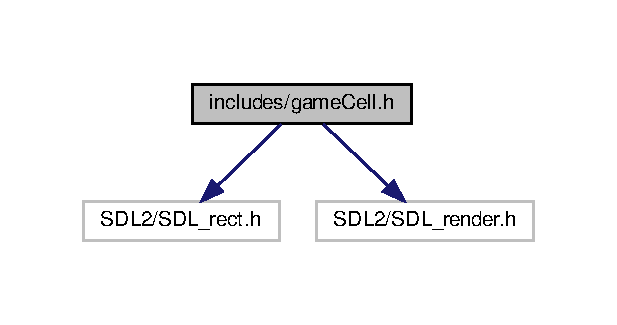
\includegraphics[width=296pt]{game_cell_8h__incl}
\end{center}
\end{figure}
This graph shows which files directly or indirectly include this file\+:
\nopagebreak
\begin{figure}[H]
\begin{center}
\leavevmode
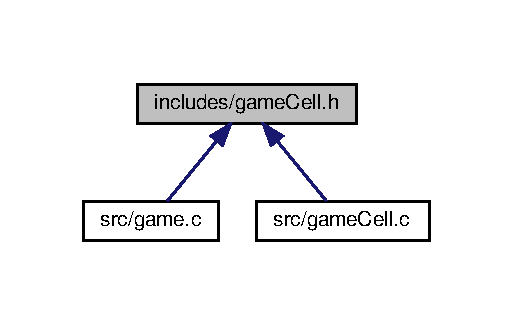
\includegraphics[width=246pt]{game_cell_8h__dep__incl}
\end{center}
\end{figure}
\subsection*{Data Structures}
\begin{DoxyCompactItemize}
\item 
struct \hyperlink{structgame_cell}{game\+Cell}
\end{DoxyCompactItemize}
\subsection*{Typedefs}
\begin{DoxyCompactItemize}
\item 
\mbox{\Hypertarget{game_cell_8h_a898bd037fbdd4d79f7b7dbbb81118c2b}\label{game_cell_8h_a898bd037fbdd4d79f7b7dbbb81118c2b}} 
typedef struct \hyperlink{structgame_cell}{game\+Cell} {\bfseries t\+\_\+game\+Cell}
\end{DoxyCompactItemize}
\subsection*{Enumerations}
\begin{DoxyCompactItemize}
\item 
enum \hyperlink{game_cell_8h_a38e97bf4503f8099c49fac77b951ae63}{cell\+State} \{ \newline
{\bfseries N\+E\+U\+T\+R\+AL}, 
{\bfseries H\+O\+V\+E\+R\+ED}, 
{\bfseries W\+A\+T\+ER}, 
{\bfseries D\+E\+S\+T\+R\+O\+Y\+ED}, 
\newline
{\bfseries V\+A\+L\+ID}, 
{\bfseries S\+H\+IP}, 
{\bfseries I\+N\+V\+A\+L\+ID}
 \}
\end{DoxyCompactItemize}
\subsection*{Functions}
\begin{DoxyCompactItemize}
\item 
\hyperlink{structgame_cell}{t\+\_\+game\+Cell} \hyperlink{game_cell_8h_a7bdabe24007f1d273afcfd94fad6a4bf}{create\+Game\+Cell} (int, int, int, int)
\item 
void \hyperlink{game_cell_8h_a59489fd4131c2c63386102c5cc1bd561}{render\+Game\+Cell} (S\+D\+L\+\_\+\+Renderer $\ast$, \hyperlink{structgame_cell}{t\+\_\+game\+Cell} $\ast$)
\item 
void \hyperlink{game_cell_8h_ac554501d8635168e511e9ede5bc3ecfb}{set\+Game\+Cell\+State} (enum \hyperlink{game_cell_8h_a38e97bf4503f8099c49fac77b951ae63}{cell\+State}, \hyperlink{structgame_cell}{t\+\_\+game\+Cell} $\ast$)
\item 
void \hyperlink{game_cell_8h_a1add810252b8a59950263828a6d25f9d}{set\+Game\+Cell\+Ship} (u\+\_\+int8\+\_\+t, \hyperlink{structgame_cell}{t\+\_\+game\+Cell} $\ast$)
\end{DoxyCompactItemize}


\subsection{Detailed Description}
Déclaration pour les cases de jeu. 

\begin{DoxyAuthor}{Author}
Thomas De Maen 
\end{DoxyAuthor}
\begin{DoxyVersion}{Version}
1.\+0 
\end{DoxyVersion}
\begin{DoxyDate}{Date}
14 Janvier 2020
\end{DoxyDate}
Il s\textquotesingle{}agit du fichier de délaration des différentes structures de données et fonctions utilisées pour le bon fonctionnement des cases de jeu. 

\subsection{Enumeration Type Documentation}
\mbox{\Hypertarget{game_cell_8h_a38e97bf4503f8099c49fac77b951ae63}\label{game_cell_8h_a38e97bf4503f8099c49fac77b951ae63}} 
\index{game\+Cell.\+h@{game\+Cell.\+h}!cell\+State@{cell\+State}}
\index{cell\+State@{cell\+State}!game\+Cell.\+h@{game\+Cell.\+h}}
\subsubsection{\texorpdfstring{cell\+State}{cellState}}
{\footnotesize\ttfamily enum \hyperlink{game_cell_8h_a38e97bf4503f8099c49fac77b951ae63}{cell\+State}}

L\textquotesingle{}ensemble des états que peuvent avoir une case de jeu 

Definition at line 21 of file game\+Cell.\+h.



\subsection{Function Documentation}
\mbox{\Hypertarget{game_cell_8h_a7bdabe24007f1d273afcfd94fad6a4bf}\label{game_cell_8h_a7bdabe24007f1d273afcfd94fad6a4bf}} 
\index{game\+Cell.\+h@{game\+Cell.\+h}!create\+Game\+Cell@{create\+Game\+Cell}}
\index{create\+Game\+Cell@{create\+Game\+Cell}!game\+Cell.\+h@{game\+Cell.\+h}}
\subsubsection{\texorpdfstring{create\+Game\+Cell()}{createGameCell()}}
{\footnotesize\ttfamily create\+Game\+Cell (\begin{DoxyParamCaption}\item[{int}]{x,  }\item[{int}]{y,  }\item[{int}]{w,  }\item[{int}]{h }\end{DoxyParamCaption})}

Fonction permettant de créer une nouvelle case de jeu 
\begin{DoxyParams}{Parameters}
{\em x} & La coordonnée X de la case \\
\hline
{\em y} & La coordonnée Y de la case \\
\hline
{\em w} & La largeur de la case \\
\hline
{\em h} & La hauteur de la case \\
\hline
\end{DoxyParams}
\begin{DoxyReturn}{Returns}
La case qui a été créée 
\end{DoxyReturn}


Definition at line 3 of file game\+Cell.\+c.

\mbox{\Hypertarget{game_cell_8h_a59489fd4131c2c63386102c5cc1bd561}\label{game_cell_8h_a59489fd4131c2c63386102c5cc1bd561}} 
\index{game\+Cell.\+h@{game\+Cell.\+h}!render\+Game\+Cell@{render\+Game\+Cell}}
\index{render\+Game\+Cell@{render\+Game\+Cell}!game\+Cell.\+h@{game\+Cell.\+h}}
\subsubsection{\texorpdfstring{render\+Game\+Cell()}{renderGameCell()}}
{\footnotesize\ttfamily render\+Game\+Cell (\begin{DoxyParamCaption}\item[{S\+D\+L\+\_\+\+Renderer $\ast$}]{p\+Rend,  }\item[{\hyperlink{structgame_cell}{t\+\_\+game\+Cell} $\ast$}]{p\+Cell }\end{DoxyParamCaption})}

Fonction permettant de dessiner une case de jeu à l\textquotesingle{}écran, la couleur de la case dépend de son état 
\begin{DoxyParams}{Parameters}
{\em p\+Rend} & Pointeur sur le renderer S\+DL utilisé pour dessiner sur la fenêtre de jeu \\
\hline
{\em p\+Cell} & Pointeur sur la case à dessiner \\
\hline
\end{DoxyParams}


Definition at line 17 of file game\+Cell.\+c.

\mbox{\Hypertarget{game_cell_8h_a1add810252b8a59950263828a6d25f9d}\label{game_cell_8h_a1add810252b8a59950263828a6d25f9d}} 
\index{game\+Cell.\+h@{game\+Cell.\+h}!set\+Game\+Cell\+Ship@{set\+Game\+Cell\+Ship}}
\index{set\+Game\+Cell\+Ship@{set\+Game\+Cell\+Ship}!game\+Cell.\+h@{game\+Cell.\+h}}
\subsubsection{\texorpdfstring{set\+Game\+Cell\+Ship()}{setGameCellShip()}}
{\footnotesize\ttfamily set\+Game\+Cell\+Ship (\begin{DoxyParamCaption}\item[{u\+\_\+int8\+\_\+t}]{has\+Ship,  }\item[{\hyperlink{structgame_cell}{t\+\_\+game\+Cell} $\ast$}]{p\+Cell }\end{DoxyParamCaption})}

Permet de définir qu\textquotesingle{}une case possède un morceau de navir. Le premier paramètre doit être égal à 1 ou 0 
\begin{DoxyParams}{Parameters}
{\em has\+Ship} & 0 si la case ne doit pas contenir de bâteau, n\textquotesingle{}importe quel autre nombre sinon \\
\hline
{\em p\+Cell} & Pointeur sur la case sur laquelle on souhaite ajouter ou supprimer un bâteau \\
\hline
\end{DoxyParams}


Definition at line 50 of file game\+Cell.\+c.

\mbox{\Hypertarget{game_cell_8h_ac554501d8635168e511e9ede5bc3ecfb}\label{game_cell_8h_ac554501d8635168e511e9ede5bc3ecfb}} 
\index{game\+Cell.\+h@{game\+Cell.\+h}!set\+Game\+Cell\+State@{set\+Game\+Cell\+State}}
\index{set\+Game\+Cell\+State@{set\+Game\+Cell\+State}!game\+Cell.\+h@{game\+Cell.\+h}}
\subsubsection{\texorpdfstring{set\+Game\+Cell\+State()}{setGameCellState()}}
{\footnotesize\ttfamily set\+Game\+Cell\+State (\begin{DoxyParamCaption}\item[{enum \hyperlink{game_cell_8h_a38e97bf4503f8099c49fac77b951ae63}{cell\+State}}]{state,  }\item[{\hyperlink{structgame_cell}{t\+\_\+game\+Cell} $\ast$}]{p\+Cell }\end{DoxyParamCaption})}

Permet de modifier l\textquotesingle{}état d\textquotesingle{}une case. Une case détruite (D\+E\+S\+T\+R\+O\+Y\+ED ou W\+A\+T\+ER) ne peut plus changer d\textquotesingle{}état réduisant ainsi l\textquotesingle{}espace de jeu. 
\begin{DoxyParams}{Parameters}
{\em state} & Le nouvel état de la case \\
\hline
{\em p\+Cell} & Pointeur sur la case dont on souhaite modifier l\textquotesingle{}état \\
\hline
\end{DoxyParams}


Definition at line 45 of file game\+Cell.\+c.


%--- End generated contents ---

% Index
\backmatter
\newpage
\phantomsection
\clearemptydoublepage
\addcontentsline{toc}{chapter}{Index}
\printindex

\end{document}
